%    Part: Distribution
% Chapter: Anaconda progress - Framework
% ------------------------------------------------------------
% $Id: framework.tex 6207 2010-08-05 13:11:13Z al $
% ------------------------------------------------------------
    \section{Identity}
\hypertarget{sec:Distribution:Anaconda:Progress:Identity}{}
      \label{sec:Distribution:Anaconda:Progress:Identity}

\begin{description}
\item[framework:] trunk/Identity/Themes/\$THEME/Distro/Anaconda/Progress/
\end{description}

\noindent Anaconda progress identity's framework is stored here.
Anaconda progress identity's framework is illustrated in
\autoref{fig:Distribution:Anaconda:Progress:Identity} and described in
the following sections.

\begin{figure}
\hrulefill
\begin{verbatim}
trunk/Identity/Themes/$THEME/Distro/Anaconda/Progress/
|-- img
|   |-- 3
|   |   |-- bn_IN
|   |   |   |-- 01-welcome.png
|   |   |   |-- 02-donate.png
|   |   |   |-- 03-yum.png
|   |   |   `-- ... (more bn_IN language-specific images)
|   |   |-- cs
|   |   |   |-- 01-welcome.png
|   |   |   |-- 02-donate.png
|   |   |   |-- 03-yum.png
|   |   |   `-- ... (more cs language-specific images)
|   |   |-- ... (more languages here)
|   |   |-- first-lowres.png
|   |   |-- first.png
|   |   |-- ... (more language directories)
|   |   |-- progress_first-lowres.png
|   |   |-- progress_first.png
|   |   `-- ... (more language directories)
|   |-- 4
|   |-- 5
|   `-- ... (more release directories)
|-- render.sh
`-- tpl
    |-- first-lowres.svg
    |-- first.svg
    |-- list.svg
    `-- paragraph.svg
\end{verbatim}
\hrulefill
\caption{Anaconda progress identity's framework.%
   \label{fig:Distribution:Anaconda:Progress:Identity}}
\end{figure}

% ------------------------------------------------------------
 \subsection{Design Templates}
\hypertarget{sec:Distribution:Anaconda:Progress:Identity:Templates}{}
      \label{sec:Distribution:Anaconda:Progress:Identity:Templates}

\begin{description}
\item[framework:] trunk/Identity/Themes/\$THEME/Distro/Anaconda/Progress/Tpl/
\end{description}

\noindent Anaconda progress design templates are stored here.
Anaconda progress design templates are organized in: Anaconda progress
first slide and Anaconda progress language-specific slides set of
images.

Anaconda progress first slide is the one used to open the package
installation process.  Anaconda progress first slide design has no
translation. It is used just as it is, no matter what the current
Anaconda's installation language be.  Anaconda progress first slide
design is controlled by \texttt{first.svg}, and
\texttt{first-lowres.svg} design templates
(\autoref{fig:Distribution:Anaconda:Progress:Identity:Models:First}).
If the screen resolution is less than 800 x 600 pixels, the
\texttt{first-lowres.svg} design is used. If the screen resolution is
equal or greater that 800 x 600 pixels, the \texttt{first.svg} design
is used.

Anaconda progress language-specific slides set of images start to
rotate a few seconds after progress first slide.  Anaconda progress
language-specific slides set of images design is defined by
\texttt{list.svg}
(\autoref{fig:Distribution:Anaconda:Progress:Identity:Models:Paragraph})
and \texttt{paragraph.svg}
(\autoref{fig:Distribution:Anaconda:Progress:Identity:Models:List})
design templates. 

Anaconda progress language-specific slides set of images resumes
relevant features coming on the CentOS distribution that is being
installed.  As graphic designer, you need not to care very much about
translating Anaconda progress language-specific slides set of images,
this is job for translators.  As graphic designer, most of your
attention is focused on how the slides set of images looks like.

Anaconda progress language-specific slides set of images are loaded
based on Anaconda's installation language.  By default, Anaconda's
installation language is English. But you can change Anaconda's
default language in the screen ``Installation Language'' to whatever
your preferred language be. 

If Anaconda's installation language is English, Anaconda progress
language-specific slides set of images are loaded in English.  If
Anaconda's installation language is different from English, Anaconda
looks for the language-specific slides set of images that matches the
current Anaconda's installation language and uses them in the
rotation, if that slides set of images exists of course.  If there is
no language-specific slides set of images available for the current
Anaconda's installation language, Anaconda uses the English slides set
of images.

To verify the final look and feel of your Anaconda progress slide
images, you need to render them. To render Anaconda progress slide
images you use the \texttt{render.sh} identity script as described in
``\hyperlink{sec:Distribution:Anaconda:Progress:Identity:Image:Rendering}{Image
Files Rendering}''
(\autoref{sec:Distribution:Anaconda:Progress:Identity:Image:Rendering}).
The \texttt{render.sh} identity script helps you automate the
rendering process of Anaconda progress slide images.

% ------------------------------------------------------------
 \subsection{Design Models}
\hypertarget{sec:Distribution:Anaconda:Progress:Identity:Models}{}
      \label{sec:Distribution:Anaconda:Progress:Identity:Models}

\begin{description}
\item[framework:] trunk/Identity/Models/Tpl/Distro/Anaconda/Progress/
\end{description}

\noindent Anaconda progress design models are stored here.  Anaconda
progress design models are described in
\autoref{fig:Distribution:Anaconda:Progress:Identity:Models:Slides},
\autoref{fig:Distribution:Anaconda:Progress:Identity:Models:Release},
\autoref{fig:Distribution:Anaconda:Progress:Identity:Models:First},
\autoref{fig:Distribution:Anaconda:Progress:Identity:Models:Paragraph},
and \autoref{fig:Distribution:Anaconda:Progress:Identity:Models:List}.

\begin{figure}[!hbp]
\begin{center}
\fbox{\includegraphics[width=0.8\textwidth]{%
../Identity/Models/Img/en/Distro/Anaconda/Progress/view-1.pdf}}
\end{center}
\caption[Anaconda progress design model]{Anaconda progress design\
model. A = ``Header'', B = ``Slide rotation'', C =\
``Action/Navigation''.%
   \label{fig:Distribution:Anaconda:Progress:Identity:Models:Slides}}
\end{figure}

\begin{figure}[!hbp]
\begin{center}
\fbox{\includegraphics[width=0.8\textwidth]{%
../Identity/Models/Img/en/Distro/Anaconda/Progress/view-2.pdf}}
\end{center}
\caption[Anaconda progress release notes]{Anaconda progress release\
notes. A = ``Release notes'', B = ``Action/Navigation''.%
   \label{fig:Distribution:Anaconda:Progress:Identity:Models:Release}}
\end{figure}


\begin{figure}[!hbp]
\begin{center}
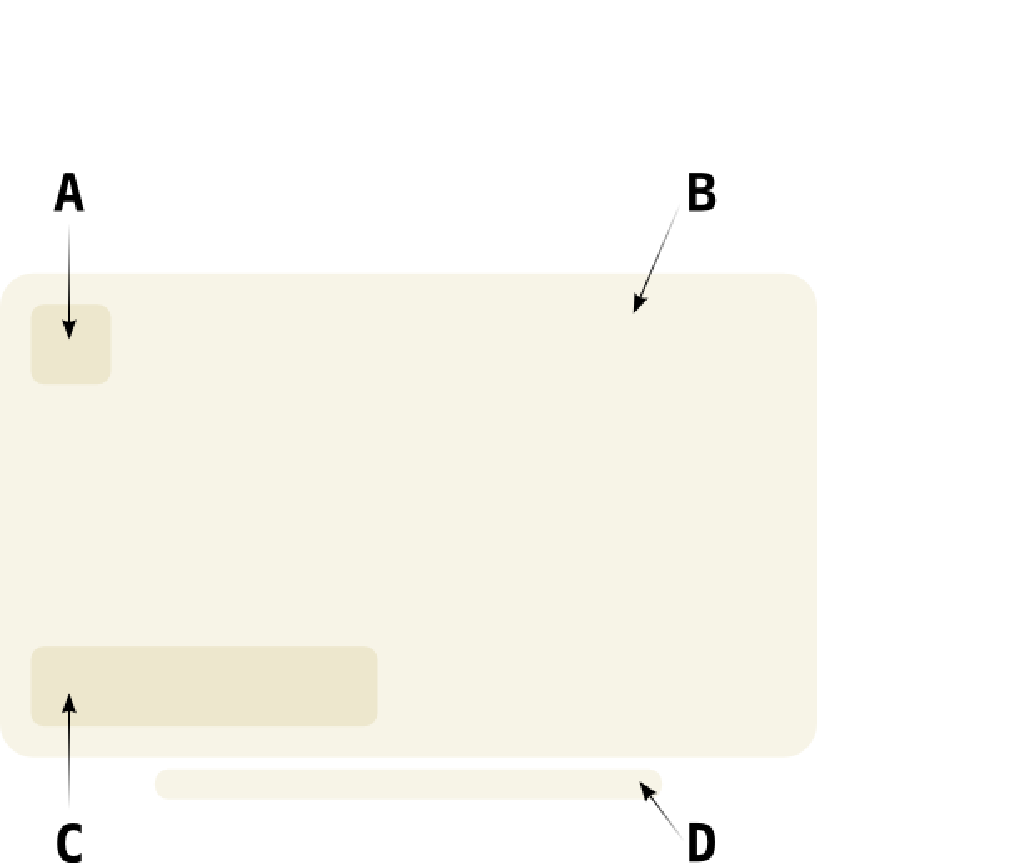
\includegraphics[width=0.8\textwidth]{%
../Identity/Models/Img/en/Distro/Anaconda/Progress/first.pdf}
\end{center}
\caption[Anaconda progress first slide template]{Anaconda progress\
first slide template. A = ``The CentOS Symbol'', B = ``The CentOS\
Default Artistic Motif'', C = ``The CentOS Release Brand'', D = ``The\
CentOS Copyright''.%
   \label{fig:Distribution:Anaconda:Progress:Identity:Models:First}}
\end{figure}

\begin{figure}[!hbp]
\begin{center}
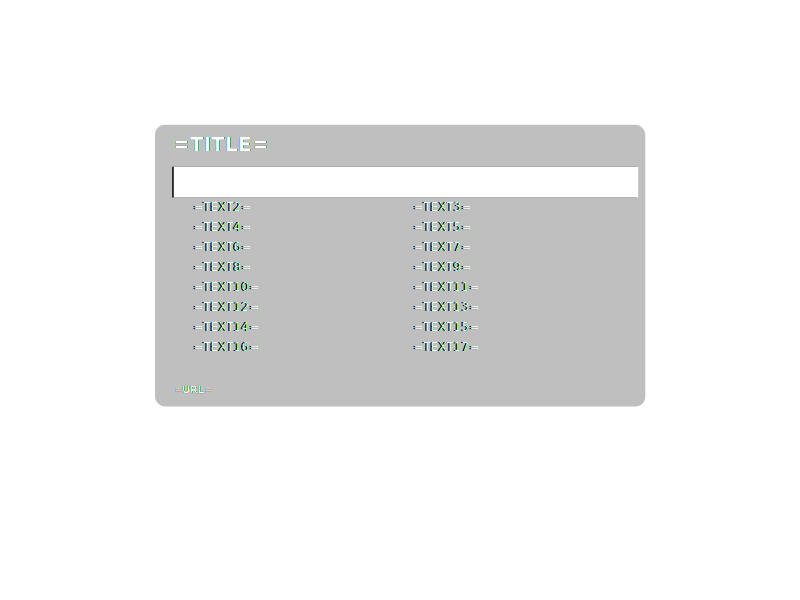
\includegraphics[width=0.8\textwidth]{%
../Identity/Models/Img/en/Distro/Anaconda/Progress/list.pdf}
\end{center}
\caption{Anaconda progress list template.%
   \label{fig:Distribution:Anaconda:Progress:Identity:Models:Paragraph}}
\end{figure}

\begin{figure}[!hbp]
\begin{center}
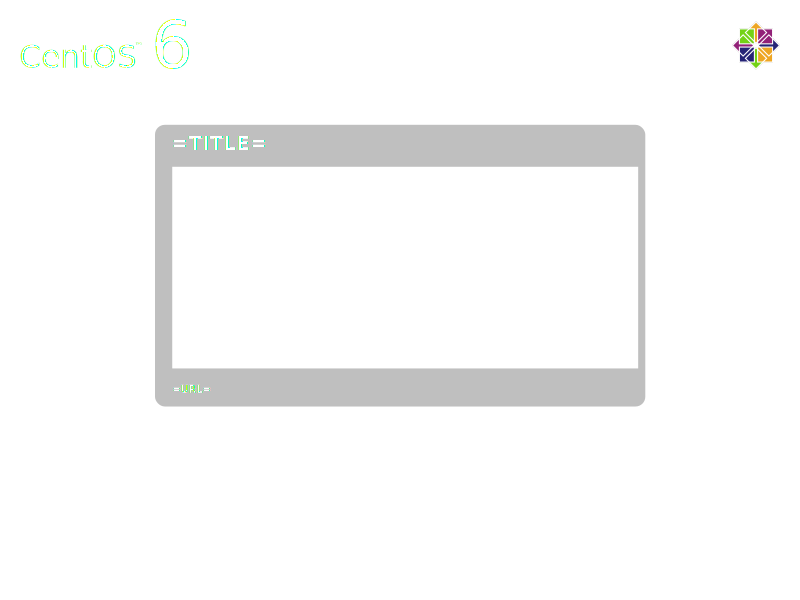
\includegraphics[width=0.8\textwidth]{%
../Identity/Models/Img/en/Distro/Anaconda/Progress/paragraph.pdf}
\end{center}
\caption{Anaconda progress paragraph template.%
   \label{fig:Distribution:Anaconda:Progress:Identity:Models:List}}
\end{figure}

% ------------------------------------------------------------
 \subsection{Image Files}
\hypertarget{sec:Distribution:Anaconda:Progress:Identity:Image}{}
      \label{sec:Distribution:Anaconda:Progress:Identity:Image}

\begin{description}
\item[framework:] trunk/Identity/Themes/\$THEME/Distro/Anaconda/Progress/Img/
\end{description}

\noindent Anaconda progress final images are stored here.

% ------------------------------------------------------------
 \subsection{Image Files Rendering}
\hypertarget{sec:Distribution:Anaconda:Progress:Identity:Image:Rendering}{}
      \label{sec:Distribution:Anaconda:Progress:Identity:Image:Rendering}

\begin{description}
\item[framework:] trunk/Identity/Themes/\$THEME/Distro/Anaconda/Progress/
\end{description}

\noindent Here is where you produce Anaconda progress slide images.
Take a look at the following rendering examples based on the
translation path shown in
\autoref{fig:Distribution:Anaconda:Progress:Translations}:\\
\\
\fbox{\texttt{./render.sh}}\\
\\
\fbox{\texttt{./render.sh '5'}}\\
\\
\fbox{\texttt{./render.sh '(3|4|5)'}}\\
\\
\fbox{\texttt{./render.sh '5/(progress|first|en)'}}\\
\\
\fbox{\texttt{./render.sh '(4|5)/(progress|first|en|es)'}}\\
\\
\fbox{\texttt{./render.sh '(4|5)/(en|es)/01-welcome'}}

% ------------------------------------------------------------
    \section{Translations}
\hypertarget{sec:Distribution:Anaconda:Progress:Translations}{}
      \label{sec:Distribution:Anaconda:Progress:Translations}{}

\begin{description}
\item[framework:] trunk/Translations/Identity/Themes/Distro/Anaconda/Progress/
\end{description}

\noindent Here is where translators locale Anaconda progress
language-specific slide set of images. Anaconda progress translation
framework is illustrated in
\autoref{fig:Distribution:Anaconda:Progress:Translations}.  Anaconda
progress translation framework defines the Anaconda progress slide
images translation path.  The translation path shown in
\autoref{fig:Distribution:Anaconda:Progress:Translations} is an
incomplet version of the real one.  It was cropped in the sake of
keeping it in just one page.  To make yourself a better idea of the
real Anaconda progress translation path, check the one inside your
working copy of CentOS Artwork Repository. That is the one you should
use in order to build your REGEX patterns when rendering Anaconda
progress slide images.

\begin{figure}
\hrulefill
\begin{verbatim}
trunk/Translations/Identity/Themes/Distro/Anaconda/Progress/
|-- 3
|   |-- bn_IN
|   |   |-- 01-welcome.sed
|   |   |-- 02-donate.sed
|   |   |-- 03-yum.sed
|   |   `-- ... (more bn_IN translation files)
|   |-- ... (more language directories)
|   |-- first-lowres.sed
|   |-- first.sed
|   |-- ... (more language directories)
|   |-- progress_first-lowres.sed
|   |-- progress_first.sed
|   `-- ... (more language directories)
|-- 4
|-- 5
|-- ... (more release directories)
|-- render.sh
`-- tpl
    |-- bn_IN
    |   |-- 01-welcome.sed
    |   |-- 02-donate.sed
    |   |-- 03-yum.sed
    |   `-- ... (more bn_IN translation files)
    |-- ... (more language directories)
    |-- first-lowres.sed
    |-- first.sed
    |-- ... (more language directories)
    |-- progress_first-lowres.sed
    |-- progress_first.sed
    `-- ... (more language directories)
\end{verbatim}
\hrulefill
\caption{Anaconda progress translation framework.%
   \label{fig:Distribution:Anaconda:Progress:Translations}}
\end{figure}

% ------------------------------------------------------------
 \subsection{Translation Markers}
\hypertarget{sec:Distribution:Anaconda:Progress:Translations:Markers}{}
      \label{sec:Distribution:Anaconda:Progress:Translations:Markers}

In Anaconda progress, translation files and design templates use the
translation markers specified in
\autoref{tab:Distribution:Identity:Markers}. 

\begin{table}[!hbp]
\centering
\begin{tabular}{ll}
\hline
\textbf{Marker}& \textbf{Description}\\
\hline
=TITLE=          & Slide's title.\\
=DESCRIPTION=    & Slide's list description.\\
=TEXT1-12=       & Slide's content.\\
=URL=            & Slide's URL.\\
=COPYRIGHT=      & Copyright notice.\\
=RELEASE=        & CentOS Distribution full release number.\\
=MAJOR\_RELEASE= & CentOS Distribution major release number.\\
=MINOR\_RELEASE= & CentOS Distribution update release number.\\
\hline
\end{tabular}
\caption{Anaconda progress translation markers.%
   \label{tab:Distribution:Identity:Markers}}
\end{table}

% ------------------------------------------------------------
    \section{Manuals}
\hypertarget{sec:Distribution:Anaconda:Progress:Manuals}{}
      \label{sec:Distribution:Anaconda:Progress:Manuals}

\begin{description}
\item[framework:] trunk/Manuals/Distribution/Anaconda/Progress/
\end{description}

\noindent Anaconda progress documentation files are prepared here.  If
you want to help improving Anaconda progress documentation this is
where you need to go.

% ------------------------------------------------------------
    \section{Scripts}
\hypertarget{sec:Distribution:Anaconda:Progress:Scripts}{}
      \label{sec:Distribution:Anaconda:Progress:Scripts}

\begin{description}
\item[framework:] trunk/Scripts/Config/Identity/Themes/Distro/Anaconda/Progress/
\end{description}

\noindent Here is stored the Anaconda progress \texttt{render.conf.sh}
configuration script.  To render Anaconda progress slide images
correctly, the \texttt{ARTCOMP} configuration variable inside Anaconda
progress configuration script should be defined as illustrated in
\autoref{fig:Distribution:Anaconda:Progress:Scripts:Config}. 

\begin{figure}
\hrulefill
\begin{verbatim}
# Define artwork component.
ARTCOMP='Distro/Anaconda/Progress'
\end{verbatim}
\hrulefill
\caption{Anaconda progress configuration layout.%
   \label{fig:Distribution:Anaconda:Progress:Scripts:Config}}
\end{figure}

